%%%%%%%%%%%%%%%%%%%%%%%%%%%%%%%%%%%%%%%%%%%%%%%%%%%%%%%%%%%%%%%%%%%%%%
%%  Copyright by Wenliang Du.                                       %%
%%  This work is licensed under the Creative Commons                %%
%%  Attribution-NonCommercial-ShareAlike 4.0 International License. %%
%%  To view a copy of this license, visit                           %%
%%  http://creativecommons.org/licenses/by-nc-sa/4.0/.              %%
%%%%%%%%%%%%%%%%%%%%%%%%%%%%%%%%%%%%%%%%%%%%%%%%%%%%%%%%%%%%%%%%%%%%%%

\newcommand{\commonfolder}{../../common-files}
\documentclass[11pt]{article}

\usepackage[most]{tcolorbox}
\usepackage{times}
\usepackage{epsf}
\usepackage{epsfig}
\usepackage{amsmath, alltt, amssymb, xspace}
\usepackage{wrapfig}
\usepackage{fancyhdr}
\usepackage{url}
\usepackage{verbatim}
\usepackage{fancyvrb}
\usepackage{adjustbox}
\usepackage{listings}
\usepackage{color}
\usepackage{subfigure}
\usepackage{cite}
\usepackage{sidecap}
\usepackage{pifont}
\usepackage{mdframed}
\usepackage{textcomp}
\usepackage{enumitem}
\usepackage{hyperref}


% Horizontal alignment
\topmargin      -0.50in  % distance to headers
\oddsidemargin  0.0in
\evensidemargin 0.0in
\textwidth      6.5in
\textheight     8.9in 

\newcommand{\todo}[1]{
\vspace{0.1in}
\fbox{\parbox{6in}{TODO: #1}}
\vspace{0.1in}
}


\newcommand{\unix}{{\tt Unix}\xspace}
\newcommand{\linux}{{\tt Linux}\xspace}
\newcommand{\minix}{{\tt Minix}\xspace}
\newcommand{\ubuntu}{{\tt Ubuntu}\xspace}
\newcommand{\setuid}{{\tt Set-UID}\xspace}
\newcommand{\openssl} {\texttt{openssl}}


\pagestyle{fancy}
\lhead{\bfseries SEED Labs}
\chead{}
\rhead{\small \thepage}
\lfoot{}
\cfoot{}
\rfoot{}


\definecolor{dkgreen}{rgb}{0,0.6,0}
\definecolor{gray}{rgb}{0.5,0.5,0.5}
\definecolor{mauve}{rgb}{0.58,0,0.82}
\definecolor{lightgray}{gray}{0.90}


\lstset{%
  frame=none,
  language=,
  backgroundcolor=\color{lightgray},
  aboveskip=3mm,
  belowskip=3mm,
  showstringspaces=false,
%  columns=flexible,
  basicstyle={\small\ttfamily},
  numbers=none,
  numberstyle=\tiny\color{gray},
  keywordstyle=\color{blue},
  commentstyle=\color{dkgreen},
  stringstyle=\color{mauve},
  breaklines=true,
  breakatwhitespace=true,
  tabsize=3,
  columns=fullflexible,
  keepspaces=true,
  escapeinside={(*@}{@*)}
}

\newcommand{\newnote}[1]{
\vspace{0.1in}
\noindent
\fbox{\parbox{1.0\textwidth}{\textbf{Note:} #1}}
%\vspace{0.1in}
}


%% Submission
\newcommand{\seedsubmission}{
Debe enviar un informe de laboratorio detallado, con capturas de pantalla, para describir lo que ha hecho y lo que ha observado.
También debe proporcionar una explicación a las observaciones que sean interesantes o sorprendentes.
Enumere también los fragmentos de código más importantes seguidos de una explicación. No recibirán créditos aquellos fragmentos de códigos que no sean explicados.}

%% Book
\newcommand{\seedbook}{\textit{Computer \& Internet Security: A Hands-on Approach}, 2nd
Edition, by Wenliang Du. Para más detalles \url{https://www.handsonsecurity.net}.\xspace}

%% Videos
\newcommand{\seedisvideo}{\textit{Internet Security: A Hands-on Approach},
by Wenliang Du. Para más detalles \url{https://www.handsonsecurity.net/video.html}.\xspace}

\newcommand{\seedcsvideo}{\textit{Computer Security: A Hands-on Approach},
by Wenliang Du. Para más detalles \url{https://www.handsonsecurity.net/video.html}.\xspace}

%% Lab Environment
\newcommand{\seedenvironment}{Este laboratorio ha sido testeado en nuestra imagen pre-compilada de una VM con Ubuntu 16.04, que puede ser descargada del sitio oficial de SEED.\xspace}

\newcommand{\seedenvironmentA}{Este laboratorio ha sido testeado en nuestra imagen pre-compilada de una VM con Ubuntu 16.04, que puede ser descargada del sitio oficial de SEED.\xspace}

\newcommand{\seedenvironmentB}{Este laboratorio ha sido testeado en nuestra imagen pre-compilada de una VM con Ubuntu 20.04, que puede ser descargada del sitio oficial de SEED .\xspace}

\newcommand{\seedenvironmentC}{Este laboratorio ha sido testeado en nuestra imagen pre-compilada de una VM con Ubuntu 20.04, que puede ser descargada del sitio oficial de SEED. Sin embargo, la mayoría de nuestros laboratorios pueden ser realizados en la nube para esto Ud. puede leer nuestra guía que explica como crear una VM de SEED en la nube.\xspace}

\newcommand{\seedenvironmentAB}{
Este laboratorio ha sido testeado en nuestras imagenes pre-compiladas de una VM con Ubuntu 16.04 y otra con Ubuntu 20.04, que pueden ser descargadas del sitio oficial de SEED.\xspace}

\newcommand{\nodependency}{Dado que utilizamos contenedores para configurar el entorno de laboratorio, este laboratorio no depende estrictamente de la VM de SEED. Puede hacer este laboratorio utilizando otras máquinas virtuales, máquinas físicas o máquinas virtuales en la nube.\xspace}

\newcommand{\adddns}{You do need to add the required IP address mapping to
the \texttt{/etc/hosts} file.\xspace}






\newcommand{\seedlabcopyright}[1]{
\vspace{0.1in}
\fbox{\parbox{6in}{\small Copyright \copyright\ {#1}\ \ by Wenliang Du.\\
      Este trabajo se encuentra bajo licencia Creative Commons.
       Attribution-NonCommercial-ShareAlike 4.0 International License.
       Si ud. remezcla, transforma y construye a partir de este material,
       Este aviso de derechos de autor debe dejarse intacto o reproducirse de una manera que sea razonable para el medio en el que se vuelve a publicar el trabajo.
       }}
\vspace{0.1in}
}






\newcommand{\telnet} {\texttt{telnet}\xspace}
\newcommand{\iptables}{\texttt{iptables}\xspace}
\newcommand{\netfilter}{\texttt{netfilter}\xspace}
\newcommand{\Netfilter}{\texttt{Netfilter}\xspace}

\newcommand{\firewallFigs}{./Figs}
\lhead{\bfseries SEED Labs -- Laboratorio Exploratorio de Firewall}

\newcommand{\pointleft}[1]{\reflectbox{\ding{217}} \textbf{\texttt{#1}}}

\begin{document}

\begin{center}
{\LARGE Laboratorio Exploratorio de Firewall}
\end{center}

\seedlabcopyright{2006 - 2021}



% *******************************************
% SECTION
% ******************************************* 
\section{Descripción}

El objetivo de este laboratorio es separado en dos partes: aprender como funciona un firewall y configurar un firewall simple para una red. Los estudiantes primero implementarán un firewall simple para filtrar paquetes, que inspeccionará los mismo y decidirá cuando rechazarlos o cuando dejarlos pasar basado en una serie de reglas del firewall.
Usando esta implementación los estudiantes podrán conocer las ideas básicas del funcionamiento de un firewall.

En la actualidad, los sistemas linux tienen integrado un firewall, basado en \texttt{netfilter}. Este firewall se llama \iptables. 
Los estudiantes tendrán disponible una topología de red simple, y serán los encargados de configurar reglas de firewall para proteger esta red.
Los estudiantes podrán experimentar diferentes tipos de aplicaciones usando \iptables. 

Este laboratorio cubre los siguientes tópicos:


\begin{itemize}[noitemsep]
\item Firewall
\item Netfilter
\item Módulo de Kernel (LKM)
\item Usando \iptables para reglas de firewall
\item Varios aplicaciones de \iptables
\end{itemize}


\paragraph{Lecturas y Videos.}
Para una cobertura más detallada sobre firewalls puede consultar:

\begin{itemize}
\item Capítulo 17 del libro de SEED, \seedbook
\item Sección 9 del curso de SEED en Udemy, \seedisvideo
\end{itemize}


\paragraph{Entorno de Laboratorio.} \seedenvironmentC




% *******************************************
% SECTION
% ******************************************* 
\section{Setup del Entorno Usando Contenedores}

Para este laboratorio, necesitamos usar varias máquinas.
Usaremos contenedores para el setup del entorno de laboratorio.

%\begin{figure}[htb]
%\begin{center}
%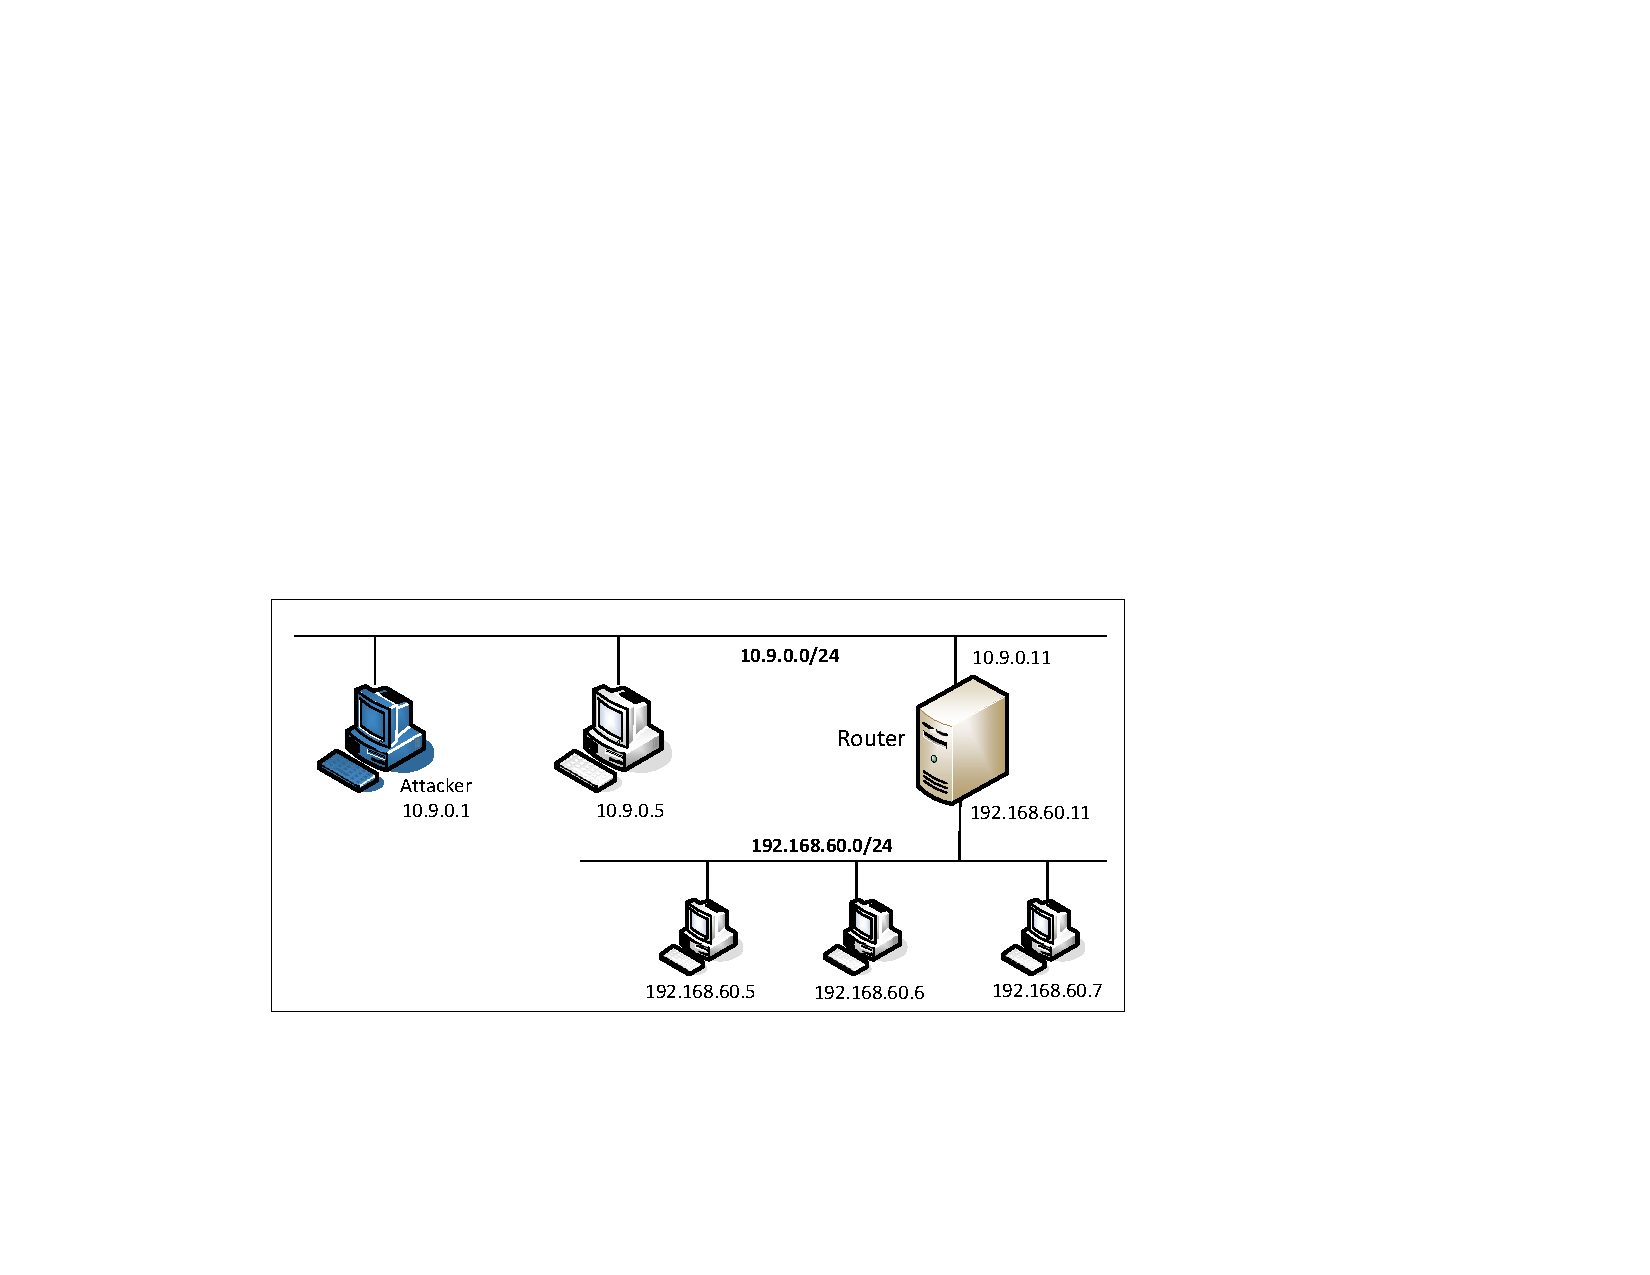
\includegraphics[width=0.8\textwidth]{./Figs/TwoLANs.pdf}
%\end{center}
%\caption{Setup del Laboratorio}
%\label{fig:labsetup}
%\end{figure}


% -------------------------------------------
% SUBSECTION
% -------------------------------------------
\subsection{Setup del Contenedor y sus Comandos}
%%%%%%%%%%%%%%%%%%%%%%%%%%%%%%%%%%%%%%%%%%%%
Para empezar a preparar el contenedor, deberá descargarse el archivo \texttt{Labsetup.zip} ubicado en el laboratorio correspondiente dentro del sitio web oficial y copiarlo dentro de la Máquina Virtual prevista por SEED. Una vez descargado deberá descomprimirlo y entrar dentro del directorio \texttt{Labsetup} donde encontrará el archivo \texttt{docker-compose.yml} que servirá para setear el entorno de laboratorio. Para una información más detallada sobre el archivo \texttt{Dockerfile} y otros archivos relacionados, puede encontrarla dentro del Manual de Usuario del laboratorio en uso, en el sitio web oficial de SEED.

Si esta es su primera experiencia haciendo el setup del laboratorio usando contenedores es recomendable que lea el manual anteriormente mencionado.

A continuación, se muestran los comandos más usados en Docker y Compose.
Debido a que estos comandos serán usados con mucha frecuencia, hemos creados un conjunto de alias para los mismos, ubicados en del archivo \texttt{.bashrc} dentro de la Máquina Virtual provista por SEED (Ubuntu 20.04)

\begin{lstlisting}
$ docker-compose build  # Build the container image
$ docker-compose up     # Start the container
$ docker-compose down   # Shut down the container

// Aliases for the Compose commands above
$ dcbuild       # Alias for: docker-compose build
$ dcup          # Alias for: docker-compose up
$ dcdown        # Alias for: docker-compose down
\end{lstlisting}


Dado que todos los contenedores estarán corriendo en un segundo plano. Necesitamos correr comandos para interactuar con los mismos, una de las operaciones fundamentales es obtener una shell en el contenedor. 
Para este propósito usaremos \texttt{"docker ps"} para encontrar el ID del contenedor deseado y ingresaremos \texttt{"docker exec"} para correr una shell en ese contenedor.
Hemos creado un alias para ello dentro del archivo \texttt{.bashrc}

\begin{lstlisting}
$ dockps        // Alias for: docker ps --format "{{.ID}}  {{.Names}}" 
$ docksh <id>   // Alias for: docker exec -it <id> /bin/bash

// The following example shows how to get a shell inside hostC
$ dockps
b1004832e275  hostA-10.9.0.5
0af4ea7a3e2e  hostB-10.9.0.6
9652715c8e0a  hostC-10.9.0.7

$ docksh 96
root@9652715c8e0a:/#  

// Note: If a docker command requires a container ID, you do not need to 
//       type the entire ID string. Typing the first few characters will 
//       be sufficient, as long as they are unique among all the containers. 
\end{lstlisting}

En caso de problemas configurando el entorno, por favor consulte la sección ``Common Problems'' en el manual ofrecido por SEED. 


%%%%%%%%%%%%%%%%%%%%%%%%%%%%%%%%%%%%%%%%%%%%




% -------------------------------------------
% SUBSECTION
% -------------------------------------------
% It does not seem to be necessary for this lab, 
% so let's comment this out.
%\subsection{Detach the VM from \texttt{192.168.60.0/24} Network} 
%%%%%%%%%%%%%%%%%%%%%%%%%%%%%%%%%%%%%%%%%%%%
%
%\paragraph{Removing the Host VM from \texttt{192.168.60.0/24} network.}

Cuando Docker crea una red, este automáticamente hace un attach de la máquina host (es decir la Máquina Virtual) hacía la red. En este caso, la máquina host es atachada en ambas redes, por lo que tendrá la IPs \texttt{10.9.0.1} y
\texttt{192.168.60.1}.
Estoo puede crear comportamientos no deseados, procederemos a remover este tipo de configuración.

En nuestro setup, solamente queremos que la Máquina Virtual este conectada a la red \texttt{10.9.0.0/24}.
Para esto necesitamos detachar la Máquina Virtual del resto de las redes, pero no podemos desactivar la interfaz de red dado que esto afectará a todos los contenedores que se encuentren en esa red.
La solución es borrar la dirección IP de la interfaz y reconfigurar el ruteo de la misma.


\begin{lstlisting}
// Get the name of the interface 
$ ip addr

// Remove the IP address from the interface
$ sudo ip addr flush <interface-name>

// Use 10.9.0.11 as the router to access 192.168.60.0/24
$ sudo ip route add 192.168.60.0/24 via 10.9.0.11
\end{lstlisting}


%%%%%%%%%%%%%%%%%%%%%%%%%%%%%%%%%%%%%%%%%%%%


% *******************************************
% SECTION
% ******************************************* 
\section{Tarea 1: Implementando un Firewall Simple} 

En esta tarea, implementaremos un firewall simple para filtrar paquete, el mismo inspeccionará los paquetes que entren y salgan y será reforzado por las políticas establecidas por el administrador. Dado que el procesamiento de pauqetes se hace dentro del kernel, el filtrado también debe ser hecho dentro del mismo. Aunque pareciera que dicho firewall requiere modificar el kernel de \linux. En el pasado se hacía modificando y recompilando el kernel. Hoy por hoy, los sistemas operativos \linux modernos nos proveen nuevos mecanismos para facilitarnos la manipulación de los paquetes sin la necesidad de recompilar la imagen del kernel. Esos dos mecanismos son \textit{Loadable Kernel Module} (\texttt{LKM}) y \texttt{Netfilter}.



\paragraph{Notas sobre los contenedores.}
Dado que todos los contenedores comparten el mismo kernel, los módulos del kernel son globales.
Además si seteamos un modelo de kernel para un contenedor, este afectará al resto de los contenedores y al host. Por esta razón, no importa donde ud. ponga el módulo del kernel. En este laboratorio, lo haremos desde la máquina virtual host.

Otra cosa a tener en cuenta que es la dirección IP de los contenedores son virtuales.
Los paquetes que irán a esas direcciones IPs virtuales pueden que no recorran todas el mismo camino como se describe en la documentación de Netfilter.
Aunque para esta tarea, en orden de evitar confusiones, trataremos de evitar esas direcciones virtuales.
Haremos la mayoría de las tareas en la máquina virtual host. Los contenedores principalmente se utilizarán para otras tareas.

% -------------------------------------------
% SUBSECTION
% ------------------------------------------- 
\subsection{Tarea 1.A: Implementar un Módulo de Kernel Simple}

{\tt LKM} nos permite agregar un nuevo módulo en el kernel en tiempo de ejecución.
Este módulo nos permite extender funcionalidades del kernel, sin recompilarlo o reiniciar la máquina.
El filtrado de paquetes de un firewall puede ser implementado como un LKM.
En esta tarea, nos familiarizaremos con LKM.

El siguiente es un LKM. Este muestra \texttt{"Hello World!"} cuando este módulo es cargado; cuando el módulo se borra del kernel, este muestra \texttt{"Bye-bye World!"}.
Los mensajes no son impresos en pantalla; se muestran dentro del archivo \texttt{/var/log/syslog}. Puede usar el comando \texttt{"dmesg"} para visualizar los mensajes.


\begin{lstlisting}[language=C, caption=\texttt{hello.c} (included in the lab setup files)]
#include <linux/module.h>
#include <linux/kernel.h>

int initialization(void)
{
    printk(KERN_INFO "Hello World!\n");
    return 0;
}

void cleanup(void)
{
    printk(KERN_INFO "Bye-bye World!.\n");
}

module_init(initialization);
module_exit(cleanup);
\end{lstlisting}

Necesitamos crear el {\tt Makefile}, que incluye el siguiente contenido (este archivo esta incluído dentro los archivos de setup del laboratorio).
Sólo escriba {\tt make}, y el rpograma será compilado como un LKM (si ud. copia y pega lo siguiente dentro del archivo \texttt{Makefile}, asegúrese de reemplazar los espacios por tabs antes de ejecutar el comando \texttt{make}).


\begin{lstlisting}
obj-m += hello.o

all:
        make -C /lib/modules/$(shell uname -r)/build M=$(PWD) modules

clean:
        make -C /lib/modules/$(shell uname -r)/build M=$(PWD) clean
\end{lstlisting}

El módulo del kernel generado es \texttt{hello.ko}. 
Puede usar el siguiente comando para cargar el módulo, listar todos los módulos y borrar el módulo.
También puede usar \texttt{"modinfo hello.ko"} para ver información sobre un módulo específico del kernel.

\begin{lstlisting}
$ sudo insmod hello.ko     (inserting a module)
$ lsmod | grep hello       (list modules)
$ sudo rmmod hello         (remove the module)
$ dmesg                    (check the messages)
\end{lstlisting}


\paragraph{Tarea.} Por favor compile este simple LKM en su Máquina Virtual y ejecútelo. Para esta tarea, no usaremos contenedores. Por favor muestre sus resultados en el informe del laboratorio.


% -------------------------------------------
% SUBSECTION
% ------------------------------------------- 
\subsection{Tarea 1.B: Implementar un Firewall Simple usando \texttt{Netfilter}}  

En esta tarea, escribiremos nuestro programa para filtrar paquetes como un LKM y lo insertaremos dentro de la cadena de procesamientos de pauqetes en el kernel. Esto no era fácil de hacer en el pasado, antes que \netfilter fuera introducido dentro de \linux.

{\tt Netfilter} está diseñado para facilitar la manipulación de los paquetes por usuarios autorizados. Logra su objetivo implementando una serie de hooks en el kernel de \linux. Estos hooks son intertados en varios lugares, incluyendo en los caminos de entrada y salida de paquetes.
Si queremos manipular los paquetes entrantes, solamente necesitamos conectar nuestro programa (dentro de un LKM) al hook que corresponde. Una vez que llega un paquete nuestro programa será invocado. Nuestro programa puede decidir si ese paquete debería de ser bloqueado o no; mas aún, podemos modificar los paquetes en el programa.

En esta tarea, ud. necesita usar LKM y {\tt Netfilter} para implementar un módulo de filtrado de paquetes. Este módulo obtendrá las políticas del firewall desde una estructura de datos y usará esta política para decidir si los paquetes deben de ser bloquyeados o no.
Quisieramos que los estudiantes se enfoquen en la parte del filtrado, el núcleo de los firewalls, a los estudiantes se les permite hardcodear las políticas del firewall en el programa. Para una guía más detallada en como usar \texttt{Netfilter} puede consultar el Capítulo 17 del libro de SEED. 
En este documento también proveeremos guías.


\paragraph{Hookeando en \texttt{Netfilter}.} 

Usar \netfilter es relativamente sencillo. Todo lo que necesitamos hacer es hookear nuestras funciones (en el módulo kernel) a los hooks correspondientes de \netfilter. Aquí mostramos un ejemplo (el código está dentro de \path{Labsetup/packet_filter}), pero pued que no sea exactamente el mismo que se muestra en este ejemplo.
La estructura del código sigue la estructura del módulo del kernel implementado anteriormente. Cuando el módulo del kernel es agregado al kernel, la función \texttt{registerFilter()} que se encuentra en el código será invocada. Dentro de esta función, registramos dos hooks en \netfilter.

Para registrar un hook, necesita preparar una estructura de datos para el hook y setear todos los parámetros que son necesarios, el más importante es el nombre de la función (Línea \ding{202})) y el número de hook (Línea \ding{203})).
El número de hook es uno de los 5 hooks en \netfilter y la función especificada será invocada cuando un pequete llegue a este hook. En este ejemplo, cuando un paquete llega al hook \texttt{LOCAL\_IN}, la función \texttt{printInfo()} será invocada (esta función será desarrollada más adelante). Una vez que la estructura de datos para hook es preparada, atachamos el hook a \netfilter (Línea \ding{204})


\begin{lstlisting}[language=C, caption={Register hook functions to \netfilter}]
static struct nf_hook_ops hook1, hook2;

int registerFilter(void) {
   printk(KERN_INFO "Registering filters.\n");
   
   // Hook 1
   hook1.hook = printInfo;                    (*@\ding{202}@*)
   hook1.hooknum = NF_INET_LOCAL_IN;          (*@\ding{203}@*)
   hook1.pf = PF_INET;
   hook1.priority = NF_IP_PRI_FIRST;
   nf_register_net_hook(&init_net, &hook1);   (*@\ding{204}@*)

   // Hook 2
   hook2.hook = blockUDP;
   hook2.hooknum = NF_INET_POST_ROUTING;
   hook2.pf = PF_INET;
   hook2.priority = NF_IP_PRI_FIRST;
   nf_register_net_hook(&init_net, &hook2);

   return 0;
}

void removeFilter(void) {
   printk(KERN_INFO "The filters are being removed.\n");
   nf_unregister_net_hook(&init_net, &hook1);
   nf_unregister_net_hook(&init_net, &hook2);
}

module_init(registerFilter);
module_exit(removeFilter);
\end{lstlisting}

\paragraph{Nota para la Máquina Virtual de Ubuntu 20.04:}
El código en el libro de SEED fue desarrollado en Ubuntu 16.04. Necesita ser modificado levemente para que funcione en Ubuntu 20.04, el cambio está en la registración del hook y la API de des-registración. Vea la diferencia en el siguiente fragmento de código:


\begin{lstlisting}[language=C]
// Hook registration:
  nf_register_hook(&nfho);                  // For Ubuntu 16.04 VM
  nf_register_net_hook(&init_net, &nfho);   // For Ubuntu 20.04 VM

// Hook unregistration:
  nf_unregister_hook(&nfho);                // For Ubuntu 16.04 VM
  nf_unregister_net_hook(&init_net, &nfho); // For Ubuntu 20.04 VM
\end{lstlisting}
 

\paragraph{Funciones Hook.} Daremos un ejemplo de una función hook. Solamente mostrará información del paquete.
Cuando \netfilter invoca una función hook, le pasa tres argumentos a esta función, incluyendo un puntero al paquete actual (\texttt{skb}). 
En el siguiente código, Línea \ding{202} muestra como obtener el número de hook del argumento \texttt{state}.
En la Línea \ding{203}, usamos la función \texttt{ip\_hdr()} para obtener el puntero para el header IP, y entonces usamos el especificador de formato de cadena \texttt{\%pI4} para mostrar la dirección IP de origen y destino en la Línea \ding{204}.

\begin{lstlisting}[language=C, caption={An example of hook function}]
unsigned int printInfo(void *priv, struct sk_buff *skb,   
                       const struct nf_hook_state *state)
{
   struct iphdr *iph;
   char *hook;

   switch (state->hook){          (*@\ding{202}@*)
     case NF_INET_LOCAL_IN: 
          printk("*** LOCAL_IN"); break;
     .. (code omitted) ...
   }

   iph = ip_hdr(skb);             (*@\ding{203}@*)           
   printk("    %pI4  --> %pI4\n", &(iph->saddr), &(iph->daddr)); (*@\ding{204}@*)
   return NF_ACCEPT;
}
\end{lstlisting}

Si necesita obtener los encabezados para otros protocolos, puede usar la siguiente funciones que se encuentran definidas en varios archivos de encabezado. La definición de la estructura de esos encabezados pueden ser encontradas dentro del directorio \path{/lib/modules/5.4.0-54-generic/build/include/uapi/linux}, donde el número de versión del directorio es el resultado de \texttt{"uname -r"}, por lo que puede variar de acuerdo a la versión de kernel instalada.

\begin{lstlisting}[language=C]
struct iphdr   *iph   = ip_hdr(skb)    // (need to include <linux/ip.h>) 
struct tcphdr  *tcph  = tcp_hdr(skb)   // (need to include <linux/tcp.h>) 
struct udphdr  *udph  = udp_hdr(skb)   // (need to include <linux/udp.h>) 
struct icmphdr *icmph = icmp_hdr(skb)  // (need to include <linux/icmp.h>) 
\end{lstlisting}
 

\paragraph{Bloqueando paquetes.} 
También ofrecemos un ejemplo de una función hook para mostrar como bloquear un paquete, si este cumple con una condición específica. El siguiente ejemplo bloquea paquetes UDP si su IP de dirección de destino es \texttt{8.8.8.8} y el puerto de destino es \texttt{53}. Esto significa que bloqueará las consultas DNS al nameserver \texttt{8.8.8.8}. 

\begin{lstlisting}[language=C, caption={Code example: blocking UDP}]
unsigned int blockUDP(void *priv, struct sk_buff *skb,
                 const struct nf_hook_state *state)
{
   struct iphdr *iph;
   struct udphdr *udph;
   u32  ip_addr;
   char ip[16] = "8.8.8.8";

   // Convert the IPv4 address from dotted decimal to a 32-bit number
   in4_pton(ip, -1, (u8 *)&ip_addr, '\0', NULL);                  (*@\ding{202}@*)
   
   iph = ip_hdr(skb);
   if (iph->protocol == IPPROTO_UDP) {
       udph = udp_hdr(skb);                                         
       if (iph->daddr == ip_addr && ntohs(udph->dest) == 53){     (*@\ding{203}@*)
            printk(KERN_DEBUG "****Dropping %pI4 (UDP), port %d\n", 
                              &(iph->daddr), port);                 
            return NF_DROP;                                       (*@\ding{204}@*)
        }
   }
   return NF_ACCEPT;                                              (*@\ding{205}@*)
}
\end{lstlisting}

En el código anterior, la Línea \ding{202} muestra como convertir dentro del kernel, una dirección IP en formato decimal con punto (es decir una cadena, como sería \texttt{1.2.3.4}) es un binario de 32-bits (\texttt{0x01020304}), por lo que puede ser comparado con el número binario que está guardado dentro de los paquetes.
La Línea \ding{203} compara la dirección IP de destino y el número de puerto con los valores de nuestra regla. Si estos valores coinciden con los de la regla,  \texttt{NF\_DROP} será retornado a \netfilter que se encargará de dropear el paquete. En caso contrario, texttt{NF\_ACCEPT} será retornado y \netfilter dejará que el paquete continue su viaje (\texttt{NF\_ACCEPT} quiere decir que el paquete es aceptado por esta función hook; pero aún así puede ser dropeado por otra función hook).

\paragraph{Tareas.} El código completo de muestra se llama \texttt{seedFilter.c} y está incluído en los archivos del laboratorio (dentro del directorio \path{Files/packet_filter}). Por favor realize las siguientes tareas (hágalas por separado).

\begin{enumerate}
	
\item Compile el código de ejemplo usando el archivo \texttt{Makefile} que se encuentra dentro de los archivos del laboratorio.
	Cargue este código dentro del kernel y demuestre que el firewall está trabajando como se espera. Puede usar el siguiente comando para generar paquetes UDP hacia \texttt{8.8.8.8}, que son los servidores DNS de Google. Si su firewall funciona, sus peticiones serán bloqueadas; de otra forma, ud. obtendrá una respuesta.

\begin{lstlisting}
dig @8.8.8.8 www.example.com 
\end{lstlisting}
 
\item Hookee la función \texttt{printInfo} en todos los hoooks de \netfilter. Aquí están las macros de los números de hooks. 
Usando los resultados de su experimento, explique en que condiciones la función de cada uno de los hooks es invocada.

\begin{lstlisting}
NF_INET_PRE_ROUTING 
NF_INET_LOCAL_IN        
NF_INET_FORWARD 
NF_INET_LOCAL_OUT 
NF_INET_POST_ROUTING    
\end{lstlisting}


\item Implemente dos hooks más para lograr lo siguiente:
(1) prevenir que otras máquinas hagan ping a la Máquina virtual y (2) prevenir que otras máquinas puedan hacer telnet a la máquina virtual.
Por favor implemente dos funciones hooks diferentes, pero registrelas en el mismo hook \netfilter. Ud. debe de decidir que hook usar.
El puerto default de telnet es \texttt{23}. Para probarlo, puede iniciar los contenedores, ir a texttt{10.9.0.5} y ejecuitar los siguientes comandos (\texttt{10.9.0.1} es la dirección IP asignada a la Máquina Virtual; por hacer las cosas más simples, puede hardcodear esta IP en las reglas del firewall):

 
\begin{lstlisting}
ping 10.9.0.1
telnet 10.9.0.1
\end{lstlisting}
     
\end{enumerate}
 

\paragraph{Nota importante:} Dando que hemos hecho cambios en el kernel, hay altas chances que el kernel pueda crashear. Asegúrese de hacer un backup de sus archivos con frecuencia. Una de las razones más comunes por la cual el sistema puede crashear es si ud. olvida de desregistrar los hooks. Cuando un módulo es boprrado, esos hooks serán llamados pero el módulo no estará presente en el kernel. Eso causará que el sistema crashee.
Para evitar esto, asegúrese que por cada hook que ud. agrega en su módulo, agregue una línea en \texttt{removeFilter} para desregistrarlo, por lo que cuando el módulo es borrado, esos hooks también.


% *******************************************
% SECTION
% ******************************************* 
\section{Tarea 2: Experimentando Reglas en un Firewall Stateless}

En las tareas anteriores, tuvimos la chance de consturir un firewall simple usando \netfilter. Actualmente, \linux tiene un firewall integrado basado en \netfilter. Este firewall se llama \iptables. Técnicamente la parte del kernel que implementa el firewall se llama  \texttt{Xtables}, nmientras que \iptables es un programa en user-space para configurar el firewall. Sin embargo \iptables es usado a menudo para referirse a la implementación a nivel kernel y a nivel usuario.



% -------------------------------------------
% SUBSECTION
% ------------------------------------------- 
\subsection{Background of \iptables}

In this task, we will use \iptables to set up a firewall. 
The \iptables firewall is designed not only to filter packets, but also to make changes to
packets. To help manage these firewall rules for different purposes, \iptables organizes all
rules using a hierarchical structure: table, chain, and rules.
There are several tables, each specifying the main purpose of the rules as shown
in Table~\ref{firewall:table:iptables}.
For example, rules for packet filtering should be
placed in the \texttt{filter} table, while rules for making changes to packets should be placed
in the \texttt{nat} or \texttt{mangle} tables.

Each table contains several chains, each of which corresponds to a \netfilter hook. Basically,
each chain indicates where its rules are enforced. For example, rules on
the \texttt{FORWARD} chain are enforced at the \texttt{NF\_INET\_FORWARD} hook, and rules on
the \texttt{INPUT} chain are enforced at the  \texttt{NF\_INET\_LOCAL\_IN} hook.

Each chain contains a set of firewall rules that will be enforced.
When we set up firewalls, we add rules to these chains.
For example, if we would like to block all incoming \telnet traffic, we would
add a rule to the \texttt{INPUT} chain of the \texttt{filter} table.  If we
would like to redirect all incoming \telnet traffic to a different
port on a different host, basically doing port forwarding, we can add a rule to the
\texttt{INPUT} chain of the \texttt{mangle} table, as we need to make changes to packets.


\begin{table}[htb]
        \centering
%       \renewcommand{\arraystretch}{1.2}
        \caption{\iptables Tables and Chains}
        \label{firewall:table:iptables}
        \centering

        \begin{tabular}{|l|l|l|}
                \hline
                \bfseries Table & \bfseries Chain & \bfseries Functionality \\
                \hline\hline
                filter          &    \texttt{INPUT}      & Packet filtering \\
                                &    \texttt{FORWARD}    & \\
                                &    \texttt{OUTPUT}      & \\
                \hline
                nat             &   \texttt{PREROUTING}    & Modifying source or destination \\
                                &   \texttt{INPUT}      & network addresses \\
                                &   \texttt{OUTPUT}      & \\
                                &   \texttt{POSTROUTING}   & \\
                \hline
                mangle          &   \texttt{PREROUTING}    & Packet content modification \\
                                &   \texttt{INPUT}      & \\
                                &   \texttt{FORWARD}     & \\
                                &   \texttt{OUTPUT}      & \\
                                &   \texttt{POSTROUTING}   & \\
                \hline
        \end{tabular}
\end{table}


% -------------------------------------------
% SUBSECTION
% ------------------------------------------- 
\subsection{Usando \iptables}


To add rules to the chains in each table, we use the \iptables command,
which is a quite powerful command. 
Students can find the manual of \iptables by typing \texttt{"man iptables"} 
or easily find many tutorials from online. 
What makes \iptables complicated is the many command-line arguments 
that we need to provide when
using the command. However, 
if we understand the structure of these command-line arguments, 
we will find out that the command is not that complicated. 


In a typical \iptables command, we add a rule to or remove a rule 
from one of the chains in one of the tables, so we need to 
specify a table name (the default is \texttt{filter}), a chain name, 
and an operation on the chain. After that, we specify the rule, which
is basically a pattern that will be matched with each of the 
packets passing through. If there is a match, an action will be 
performed on this packet. 
The general structure of the command is depicted in the following:

\begin{lstlisting}
iptables -t <table> -<operation> <chain>  <rule>   -j <target>
         ---------- --------------------  -------  -----------
            Table          Chain           Rule      Action
\end{lstlisting}


The rule is the most complicated part of the \iptables command. 
We will provide additional information later when we use 
specific rules. In the following, we list some commonly 
used commands: 


\begin{lstlisting}
// List all the rules in a table (without line number)
iptables -t nat -L -n

// List all the rules in a table (with line number)
iptables -t filter -L -n --line-numbers


// Delete rule No. 2 in the INPUT chain of the filter table 
iptables -t filter -D INPUT 2

// Drop all the incoming packets that satisfy the <rule>
iptables -t filter -A INPUT <rule>  -j DROP
\end{lstlisting}


\paragraph{Note.} Docker relies on \iptables to manage 
the networks it creates, so it adds many rules to 
the \texttt{nat} table. 
When we manipulate \iptables rules, we should be careful 
not to remove Docker rules. For example, it will be quite
dangerous to run the \texttt{"iptables -t nat -F"} command, because 
it removes all the rules in the \texttt{nat} table,
including many of the Docker rules. That will cause 
trouble to Docker containers. Doing this for 
the \texttt{filter} table is fine, because Docker 
does not touch this table. 


% -------------------------------------------
% SUBSECTION
% -------------------------------------------
\subsection{Tarea 2.A: Protegiendo el Router} 

In this task, we will set up rules to prevent outside machines from 
accessing the router machine, except ping.   
Please execute the following \iptables
command on the router container, and then try to 
access it from \texttt{10.9.0.5}. (1) Can you ping 
the router? (2) Can you telnet into the router (a 
telnet server is running on all the containers; an
account called \texttt{seed} was created on them with
a password \texttt{dees}). 
Please report your observation and explain the purpose for 
each rule. 

\begin{lstlisting}
iptables -A INPUT  -p icmp --icmp-type echo-request -j ACCEPT
iptables -A OUTPUT -p icmp --icmp-type echo-reply   -j ACCEPT
iptables -P OUTPUT DROP     (*@\pointleft{Set default rule for OUTPUT}@*)
iptables -P INPUT  DROP     (*@\pointleft{Set default rule for INPUT}@*)
\end{lstlisting}
 

\paragraph{Cleanup.} 
Before moving on to the next task, please restore the \texttt{filter} 
table to its original state by running the following commands:

\begin{lstlisting}
iptables -F
iptables -P OUTPUT ACCEPT
iptables -P INPUT  ACCEPT
\end{lstlisting}
 
Another way to restore the states of all the tables is to restart the 
container. You can do it using the following command (you need 
to find the container's ID first):

\begin{lstlisting}
$ docker restart <Container ID>
\end{lstlisting}
 


% -------------------------------------------
% SUBSECTION
% -------------------------------------------
\subsection{Tarea 2.B: Protegiendo la Red Interna} 

In this task, we will set up firewall rules on the router to protect the 
internal network \texttt{192.168.60.0/24}. We need to use the 
FORWARD chain for this purpose. 

The directions of packets in the INPUT and OUTPUT chains are clear:
packets are either coming into (for INPUT) or going out (for OUTPUT). 
This is not true for the FORWARD chain, because it is 
bi-directional: packets going into
the internal network or going out to the external network
all go through this chain. To specify the direction,
we can add the interface options using \texttt{"-i xyz"} (coming in from 
the \texttt{xyz} interface) and/or \texttt{"-o xyz"} (going out 
from the \texttt{xyz} interface). The interfaces 
for the internal and external networks are different.
You can find out the interface names via the 
\texttt{"ip addr"} command.


In this task, we want to implement a firewall to protect the 
internal network. More specifically, we need to enforce the 
following restrictions on the ICMP traffic: 

\begin{enumerate}[noitemsep]
  \item Outside hosts cannot ping internal hosts. 
  \item Outside hosts can ping the router.
  \item Internal hosts can ping outside hosts. 
  \item All other packets between the internal and external networks should be blocked.
\end{enumerate}

You will need to use the \texttt{"-p icmp"} options to specify the match
options related to the ICMP protocol. You can run 
\texttt{"iptables -p icmp -h"} to find out all the ICMP match
options. The following example drops the ICMP echo request.


\begin{lstlisting}
iptables -A FORWARD -p icmp --icmp-type echo-request -j DROP
\end{lstlisting}

In your lab report, please include your rules and  
screenshots to demonstrate that your firewall works as expected.
When you are done with this task,
please remember to clean the table or restart the container 
before moving on to the next task.


% -------------------------------------------
% SUBSECTION
% -------------------------------------------
\subsection{Tarea 2.C: Protegiendo los Servicios Internos}

In this task, we want to protect the TCP servers 
inside the internal network (\texttt{192.168.60.0/24}). 
More specifically, we would like to achieve the following objectives.

\begin{enumerate}[noitemsep]
  \item All the internal hosts run a telnet server (listening to port \texttt{23}). 
    Outside hosts can only access the telnet server on \texttt{192.168.60.5},
    not the other internal hosts.

  \item Outside hosts cannot access other internal servers. 

  \item Internal hosts can access all the internal servers.

  \item Internal hosts cannot access external servers.

  \item In this task, the connection tracking mechanism is not allowed. 
    It will be used in a later task. 
\end{enumerate}

You will need to use the \texttt{"-p tcp"} options to specify the match
options related to the TCP protocol. You can run 
\texttt{"iptables -p tcp -h"} to find out all the TCP match
options. The following example allows the TCP packets coming from
the interface \texttt{eth0} if their source port is \texttt{5000}.  

\begin{lstlisting}
iptables -A FORWARD -i eth0 -p tcp --sport 5000  -j ACCEPT
\end{lstlisting}


When you are done with this task,
please remember to clean the table or restart the container 
before moving on to the next task.




% *******************************************
% SECTION
% ******************************************* 
\section{Tarea 3: trackeo de Conexión y Firewall Stateful}


In the previous task, we have only set up stateless firewalls, which inspect each
packet independently. However, packets
are usually not independent; they may be part of a TCP connection,
or they may be ICMP packets triggered by other packets. Treating them
independently does not take into consideration the context of the
packets, and can thus lead to inaccurate, unsafe, or complicated firewall rules.
For example, if we would like to allow TCP packets to get into our network
only if a connection was made first, we cannot achieve that easily 
using stateless packet filters, because when the firewall examines each individual TCP packet,
it has no idea whether the packet belongs to an existing connection
or not, unless the firewall maintains some state information for each connection.
If it does that, it becomes a stateful firewall.


% -------------------------------------------
% SUBSECTION
% ------------------------------------------- 
\subsection{Tarea 3.A: Experimentado con el Trackeo de Conexiones} 


To support stateful firewalls, we need to be able to track connections. 
This is achieved by the \texttt{conntrack} mechanism inside the kernel. 
In this task, we will conduct experiments related to this module, and 
get familiar with the connection tracking mechanism. 
In our experiment, we will check the connection tracking information
on the router container. This can be done using the following command: 

\begin{lstlisting}
# conntrack -L
\end{lstlisting}

The goal of the task is to use a series of experiments to 
help students understand the 
connection concept in this tracking mechanism, especially
for the ICMP and UDP protocols, because unlike TCP,  they 
do not have connections. 
Please conduct the following experiments. For each experiment, please 
describe your observation, along with your explanation. 

\begin{itemize}
\item ICMP experiment: Run the following command and 
check the connection tracking information on the router. Describe
your observation. How long is the ICMP connection state be kept? 

\begin{lstlisting}
// On 10.9.0.5, send out ICMP packets
# ping 192.168.60.5
\end{lstlisting}

\item UDP experiment: Run the following command and 
check the connection tracking information on the router. Describe
your observation. How long is the UDP connection state be kept? 


\begin{lstlisting}
// On 192.168.60.5, start a netcat UDP server
# nc -lu 9090

// On 10.9.0.5, send out UDP packets  
# nc -u 192.168.60.5 9090
<type something, then hit return>
\end{lstlisting}


\item TCP experiment: Run the following command and 
check the connection tracking information on the router. Describe
your observation. How long is the TCP connection state be kept? 

\begin{lstlisting}
// On 192.168.60.5, start a netcat TCP server
# nc -l 9090

// On 10.9.0.5, send out TCP packets 
# nc 192.168.60.5 9090
<type something, then hit return>
\end{lstlisting}

\end{itemize}
 


% -------------------------------------------
% SUBSECTION
% ------------------------------------------- 
\subsection{Tarea 3.B: Configurando un Firewall Stateful} 


Now we are ready to set up firewall rules based on connections. 
In the following example, 
the \texttt{"-m conntrack"} option indicates that we are using the \texttt{conntrack} module,
which is a very important module for \iptables; it tracks connections, and
\iptables replies on the tracking information to build stateful firewalls. 
The \texttt{--ctsate ESTABLISHED,RELATED} indicates that whether a packet
belongs to an \texttt{ESTABLISHED} or \texttt{RELATED} connection.
The rule allows TCP packets belonging to an existing connection to 
pass through. 

\begin{lstlisting}
iptables -A FORWARD -p tcp -m conntrack          \
         --ctstate ESTABLISHED,RELATED -j ACCEPT
\end{lstlisting}


The rule above does not cover the SYN packets, which do not belong to 
any established connection. Without it, we will not be able to 
create a connection in the first place. Therefore, we need to 
add a rule to accept incoming SYN packet: 

\begin{lstlisting}
iptables -A FORWARD -p tcp -i eth0 --dport 8080 --syn  \
         -m conntrack --ctstate NEW -j ACCEPT 
\end{lstlisting}

Finally, we will set the default policy on FORWARD to drop
everything. This way, if a packet is not accepted by the two
rules above, they will be dropped. 

\begin{lstlisting}
iptables -P FORWARD DROP
\end{lstlisting}


Please rewrite the firewall rules in Task 2.C, but this time,
\textbf{we will add a rule allowing internal hosts to visit any 
external server} (this was not allowed in Task 2.C). 
After you write the rules using the connection tracking mechanism, 
think about how to do it without using the connection tracking
mechanism (you do not need to actually implement them). 
Based on these two sets of rules, 
compare these two different approaches, and 
explain the advantage and disadvantage of each approach. 
When you are done with this task, remember to clear all the rules. 



% *******************************************
% SECTION
% ******************************************* 
\section{Tarea 4: Limitando el Tráfico de Red}

In addition to blocking packets, we can also 
limit the number of packets that can pass through the firewall. 
This can be done using the \texttt{limit} module of \iptables.
In this task, we will use this module to limit how many packets 
from \texttt{10.9.0.5} are allowed to get into the internal network. 
You can use \texttt{"iptables -m limit -h"} to see the manual.  

\begin{lstlisting}
$ iptables -m limit -h
limit match options:
--limit avg             max average match rate: default 3/hour
                        [Packets per second unless followed by
                        /sec /minute /hour /day postfixes]
--limit-burst number    number to match in a burst, default 5
\end{lstlisting}
 

Please run the following commands on router, and then
ping \texttt{192.168.60.5} from \texttt{10.9.0.5}.  
Describe your observation. 
Please conduct the experiment with and without the second rule, 
and then explain whether the second rule is needed or not, and why.

\begin{lstlisting}
iptables -A FORWARD -s 10.9.0.5 -m limit \
         --limit 10/minute --limit-burst 5 -j ACCEPT

iptables -A FORWARD -s 10.9.0.5 -j DROP
\end{lstlisting}



% *******************************************
% SECTION
% *******************************************
\section{Tarea 5: Balanceo de Carga}

The \iptables is very powerful. In addition to firewalls,
it has many other applications. We will not be able to 
cover all its applications in this lab, but we will experimenting
with one of the applications, load balancing. In this task,
we will use it to load balance three UDP servers running in the 
internal network. Let's first start the server
on each of the hosts: \texttt{192.168.60.5}, \texttt{192.168.60.6}, and 
\texttt{192.168.60.7} (the \texttt{-k} option indicates that 
the server can receive UDP datagrams from multiple hosts):

\begin{lstlisting}
nc -luk 8080
\end{lstlisting}

We can use the \texttt{statistic} module to achieve load balancing. 
You can type the following command to get its manual. You can 
see there are two modes: \texttt{random} and \texttt{nth}. 
We will conduct experiments using both of them.

\begin{lstlisting}
$ iptables -m statistic -h 
statistic match options:
 --mode mode         Match mode (random, nth)
 random mode:
[!] --probability p  Probability
 nth mode:
[!] --every n        Match every nth packet
 --packet p          Initial counter value (0 <= p <= n-1, default 0)
\end{lstlisting}
 

\paragraph{Using the \texttt{nth} mode (round-robin).}
On the router container, we set the following rule, which applies 
to all the UDP packets going to port \texttt{8080}. 
The \texttt{nth} mode of the \texttt{statistic} module is used; 
it implements a round-robin load balancing policy: for every
three packets, pick the packet 0 (i.e., the first one), 
change its destination IP address and port number to 
\texttt{192.168.60.5}  and \texttt{8080}, respectively.  
The modified packets will continue on its journey.

\begin{lstlisting}
iptables -t nat -A PREROUTING -p udp --dport 8080      \
         -m statistic --mode nth --every 3 --packet 0  \
         -j DNAT --to-destination 192.168.60.5:8080
\end{lstlisting}

It should be noted that those packets that do not match
the rule will continue on their journeys; they will
not be modified or blocked. With this rule in place, 
if you send a UDP packet to the router's \texttt{8080} port,  
you will see that one out of three packets gets to 
\texttt{192.168.60.5}. 

\begin{lstlisting}
// On 10.9.0.5
echo hello | nc -u 10.9.0.11 8080
<hit Ctrl-C>
\end{lstlisting}
 

Please add more rules to the router container, 
so all the three internal hosts get the equal 
number of packets. 
Please provide some explanation for the rules. 


\paragraph{Using the \texttt{random} mode.}
Let's use a different mode to achieve the load balancing. The following 
rule will select a matching packet with the probability \texttt{P}.  
You need to replace \texttt{P} with a probability number.

\begin{lstlisting}
iptables -t nat -A PREROUTING -p udp --dport 8080   \
         -m statistic --mode random --probability P \
         -j DNAT --to-destination 192.168.60.5:8080
\end{lstlisting}

Please use this mode to implement your load balancing 
rules, so each internal server get roughly the 
same amount of traffic (it may not be exactly the same, 
but should be close when the total number of packets is large). 
Please provide some explanation for the rules. 




% *******************************************
% SECTION
% ******************************************* 
\section{Informe del Laboratorio y Demostraciones}


%%%%%%%%%%%%%%%%%%%%%%%%%%%%%%%%%%%%%%%%

Debe enviar un informe de laboratorio detallado, con capturas de pantalla, para describir lo que ha hecho y lo que ha observado.
También debe proporcionar una explicación a las observaciones que sean interesantes o sorprendentes.
Enumere también los fragmentos de código más importantes seguidos de una explicación. No recibirán créditos aquellos fragmentos de códigos que no sean explicados.
%%%%%%%%%%%%%%%%%%%%%%%%%%%%%%%%%%%%%%%%

\section*{Agradecimientos}

Este documento ha sido traducido al Español por Facundo Fontana



\end{document}
%%%%%%%%%%%%%%%%%%%%%%%%%%%%%%%%%%%%%%%%%%%%%%%%%%%%%%%%
%%%%%%%%%%%%%%%%%%%%%%%%%%%%%%%%%%%%%%%%%%%%%%%%%%%%%%%%



